\documentclass{article}
\usepackage[spanish]{babel}
\usepackage[utf8]{inputenc}
\usepackage{mathtools}
\usepackage{graphicx}
\usepackage[usenames]{color}


\title{\Huge Aplicaciones de guía para personas con discapacidad visual}

\begin{document}
	
	\begin{titlepage}
		\maketitle
		\thispagestyle{empty}
	\end{titlepage}
	
	%ABSTRACT
	\begin{abstract}
	    En los últimos años ha aumentado la concienciación acerca de la importancia de desarrollar tecnologías accesibles e inclusivas, de modo que, concretamente, cada vez son más las aplicaciones que tratan de reducir las limitaciones que antes las convertían en inalcanzables para personas con discapacidad visual.
	    \\
	    A continuación haremos un pequeño estudio sobre qué apliaciones de accesibilidad ya existen en el campo de la navegación, bien sea por interiores o exteriores, y cómo funcionan.
	
	\end{abstract}
	
	%PRIMERA APP
	\section{Google Maps}
		El pasado 10 de Octubre de 2019, en el World Sight Day, Google dió a conocer la última actualización de la famosa aplicación "Google Maps". Esta incluiría una nueva característica desarrollada desde cero por y para personas con discapacidad visual que convertiría a la misma en una app accesible.
		\\
		\\
		El proyecto consiste en la implementación de una nueva funcionalidad, que facilita la posibilidad de recibir instrucciones de voz más detalladas y nuevos tipos de anuncios verbales muy útiles para las rutas de a pie.
		\\
		Algunas de las nuevas instrucciones incluídas son: informar de manera proactiva que estás en la ruta correcta, la distancia hasta el próximo giro, la dirección en la que estás caminando, avisos para cruzar con precaución si te aproximas a una gran intersección, notificaciones en caso de ser redirigido por causa de haber abandonado accidentalmente la ruta correcta, etc. De esta manera, la aplicación pretende brindar de independencia a las personas que padecen ceguera tratando de que se sientan cómodas y seguras a la hora de explorar lugares nuevos y desconocidos.
		\\
		\\
		La guía de voz detallada para la navegación está actualmente en desarrollo, estando ya disponible en inglés en los Estados Unidos y en japonés en Japón. Su soporte para otros idiomas y países sigue en camino.
		\\
		\\
		\textcolor{blue}{Link: https://blog.google/products/maps/better-maps-for-people-with-vision-impairments/}
		\\
		\\
		En cuanto al desplazamiento por interiores, Google Maps ha incluido mapas de interiores. Entre los edificios que tienen esta funcionalidad destacan los aeropuertos, centros, comerciales, estadios y los lugares con transporte público. 
		\\
		A continuación vemos un ejemplo del famoso Madison Square Garden de Nueva York: 
		
		 \begin{figure}[h!]
			\centering
			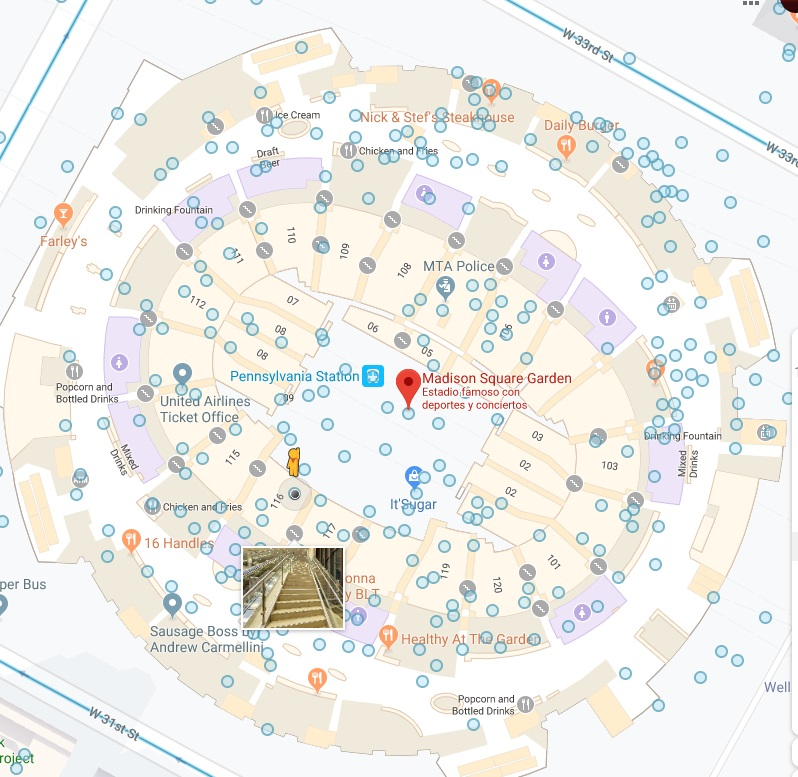
\includegraphics[width=0.6\textwidth]{MadSq2}
			\caption{Basta con ampliar para que Maps nos muestre el mapa del edificio. Arrastrando el muñequito de Google Street View podemos posicionarnos en el interior.}
			\label{fig:ejemplo}
		\end{figure}
		
		 \begin{figure}[h!]
			\centering
			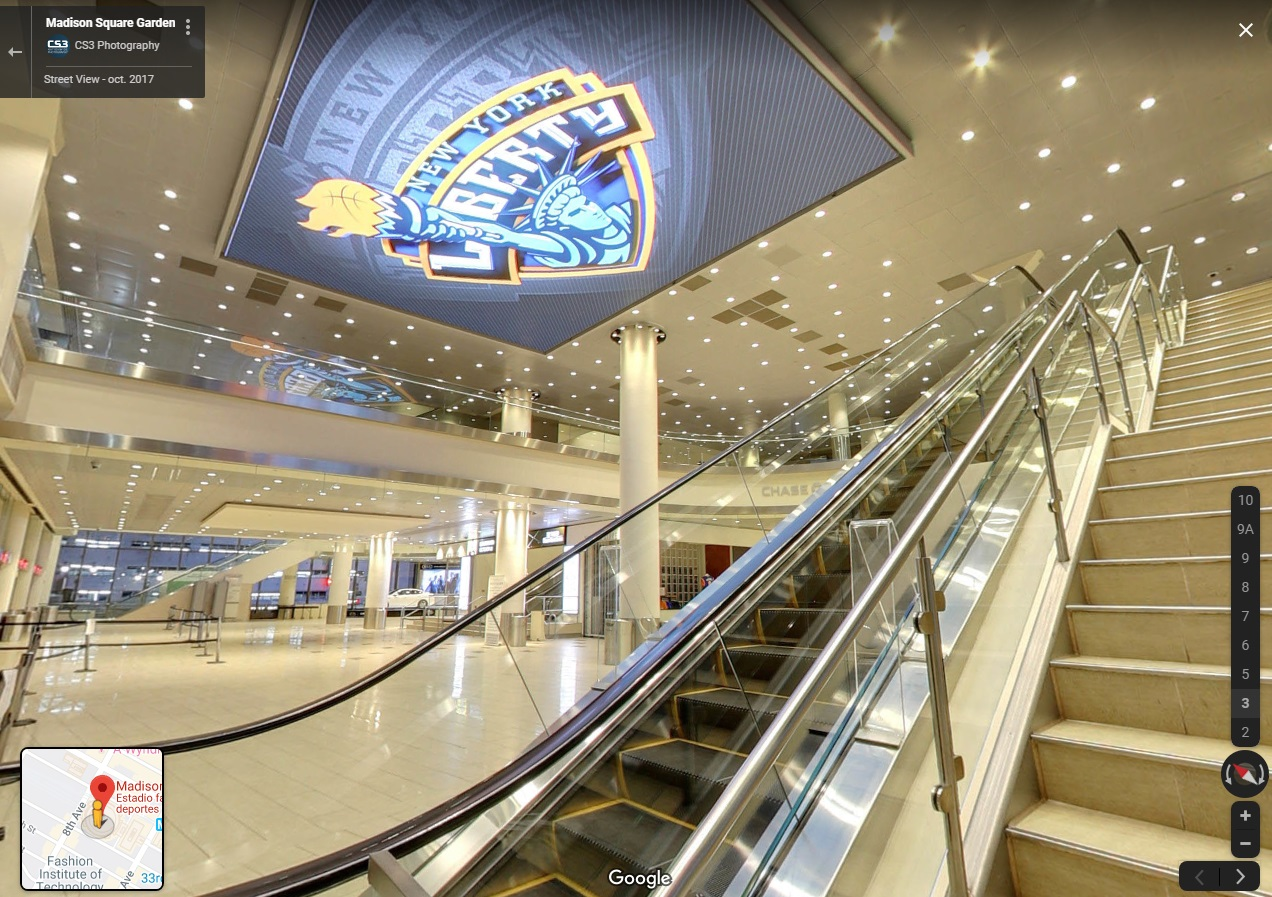
\includegraphics[width=0.6\textwidth]{MadSq3}
			\caption{Vista del interior del Madison Square Garden. }
			\label{fig:ejemplo}
		\end{figure}
	
		Desde la vista del interior puedes desplazarte por todo el edificio de la misma manera que lo haríamos con el Street View convencional aunque, no tenemos la posibilidad de buscar por información extra. Por ejemplo, localizar dónde están los baños del edificio.
		\\
		\\
		\textcolor{blue}{Link: https://www.google.es/intl/es/maps/about/partners/indoormaps/}		
		\\
		Este es un proyecto colaborativo, desde la web nos permiten actualizar planos. Además, está disponible tanto para ordenador como plataformas Android e iOS. 
	
\end{document}
© 2019 GitHub, Inc.
Terms
Privacy
Security
Status
Help
Contact GitHub
Pricing
API
Training
Blog
About

